\section{Method}
\label{sec:method}

Figure~\ref{fig:architecture} illustrates the complete \sone{} architecture, and Table~\ref{tab:params} details exact tensor counts, parameter counts, and serialized FP16 footprints across \textbf{Sone-6.5M}, \textbf{Sone-v2-Base}, and \textbf{Sone-Pro}. We formalise the bar-ruler representation and untouched master splicing (\S\ref{sec:ruler}), derive phase-coherent Dual-Axis \op{Cochlea} (\S\ref{sec:stems}), vinyl-speed equivariant \op{Tympanum} and neuro-symbolic comb-grid tracking (\S\ref{sec:ear}), \op{Cortex} and \op{Cingulate} with Best-of-$K$ reranking and vocal-onset lock (\S\ref{sec:beat}), and the zero-copy Rust/WebAssembly runtime (\S\ref{sec:runtime}).

\begin{figure*}[!tbp]
  \centering
  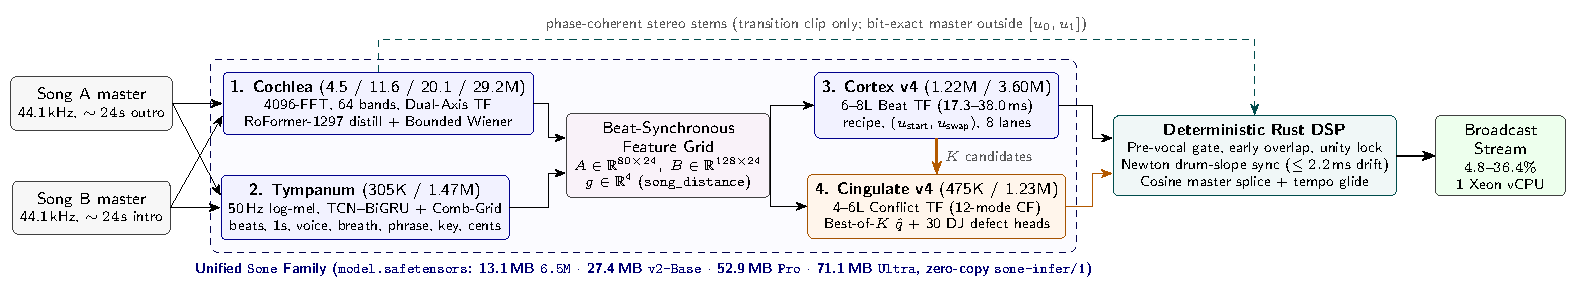
\includegraphics[width=\linewidth]{figures/architecture.pdf}
  \caption{System architecture of the \sone{} model family. Raw $44.1$\,kHz stereo boundary windows around Song~A's outro and Song~B's intro are separated by \textbf{Cochlea} ($4096$-FFT, $64$-band Dual-Axis Transformer with bounded Wiener mixture consistency) and analysed by \textbf{Tympanum} ($50$\,Hz TCN--BiGRU + multi-octave comb-grid) into a $24$-feature beat table. \textbf{Cortex} proposes transition recipes, bar offsets, and $8$ stem gain trajectories; \textbf{Cingulate} scores $K$ candidate plans across $30$ DJ defect heads; and the Rust DSP engine renders vocal-onset-locked blends spliced via raised-cosine seams into untouched master stereo outside $[u_0, u_1]$.}
  \label{fig:architecture}
\end{figure*}

\begin{table*}[t]
\centering
\caption{Exact parameter counts, tensor counts, architectural configurations, and serialized IEEE-754 FP16 \op{.safetensors} footprints across the three-tier \sone{} model family. All three tiers share the identical zero-copy \op{sone-infer/1} wire schema (\op{Sone::load}).}
\label{tab:params}
\footnotesize
\setlength{\tabcolsep}{4.0pt}
\resizebox{\linewidth}{!}{\begin{tabular}{@{}lllrrr@{}}
\toprule
Tier / Organ & Namespace & Architecture summary & Tensors & Parameters & FP16 size \\
\midrule
\textbf{Sone-6.5M} (\op{v1}) & \op{cochlea.*} & 42-band STFT ($2048/512$), $6\times$ (DWConv + Band-MHA), $d=64$, 3-stem res. & 728 & 4{,}519{,}376 & 9.10\,MB \\
 & \op{tympanum.*} & 50\,Hz log-mel ($M=128$), $4\times$ DWConv ($C=96$) + $2\times$ BiGRU ($h=64$) & 54 & 304{,}510 & 0.61\,MB \\
 & \op{cortex.*} & Beat Transformer ($209$ tok), $L=6, d=128, H=4, d_{\text{ff}}=512$ & 75 & 1{,}221{,}494 & 2.45\,MB \\
 & \op{cingulate.*} & Conflict Transformer ($209$ tok), $L=4, d=96, H=4$, 11 defect heads & 53 & 475{,}071 & 0.95\,MB \\
 & \textbf{Unified \op{v1}} & Single-file \op{sone-6.5M-f16.safetensors} ($0.13\times$ 1-vCPU Cochlea RT) & \textbf{910} & \textbf{6{,}520{,}451} & \textbf{13.12\,MB} \\
\midrule
\textbf{Sone-v2-Base} & \op{cochlea.*} & 64-band STFT ($4096/1024$), $6\times$ Dual-Axis TF ($d=80, H=4$), 4-stem Wiener & 1{,}338 & 11{,}605{,}860 & 23.33\,MB \\
 & \op{tympanum.*} & 50\,Hz log-mel ($M=128$), $4\times$ DWConv ($C=96$) + $2\times$ BiGRU ($h=64$), equiv. & 54 & 304{,}510 & 0.61\,MB \\
 & \op{cortex.*} & Beat Transformer ($209$ tok), $L=6, d=128, H=4, d_{\text{ff}}=512$ (\op{v3}) & 75 & 1{,}221{,}494 & 2.45\,MB \\
 & \op{cingulate.*} & Conflict Transformer ($209$ tok), $L=4, d=96, H=4$, 30 DJ defect heads & 53 & 475{,}071 & 0.95\,MB \\
 & \textbf{Unified \op{v2-Base}} & Single-file \op{sone-v2-base-f16.safetensors} ($0.40\times$ 1-vCPU Cochlea RT) & \textbf{1{,}520} & \textbf{13{,}606{,}935} & \textbf{27.36\,MB} \\
\midrule
\textbf{Sone-Pro} & \op{cochlea.*} & 64-band STFT ($4096/1024$), $8\times$ Dual-Axis TF ($d=128, H=8$), 4-stem Wiener & 1{,}378 & 20{,}069{,}012 & 40.26\,MB \\
 & \op{tympanum.*} & 50\,Hz log-mel ($M=160$), $6\times$ DWConv ($C=160$) + $3\times$ BiGRU ($h=128$), equiv. & 76 & 1{,}473{,}406 & 2.95\,MB \\
 & \op{cortex.*} & Beat Transformer ($209$ tok), $L=8, d=192, H=6, d_{\text{ff}}=768$ (\op{v3-Pro}) & 93 & 3{,}604{,}726 & 7.22\,MB \\
 & \op{cingulate.*} & Conflict Transformer ($209$ tok), $L=6, d=128, H=4$, 30 DJ defect heads & 71 & 1{,}225{,}247 & 2.46\,MB \\
 & \textbf{Unified \op{Pro}} & Single-file \op{sone-pro-f16.safetensors} ($0.95\times$ 1-vCPU Cochlea RT) & \textbf{1{,}618} & \textbf{26{,}372{,}391} & \textbf{52.90\,MB} \\
\bottomrule
\end{tabular}}
\end{table*}


% ---------------------------------------------------------------------------
\subsection{Bar-Ruler Representation and Untouched Master Splicing}
\label{sec:ruler}

Every transition between outgoing track~$A$ and incoming track~$B$ is parameterised on a continuous metrical coordinate $u \in \R$ measured in four-beat bars relative to \emph{the one} ($u = 0$), the downbeat where track~$B$ assumes primary rhythmic and harmonic ownership. Track~$A$ plays at its native tempo $\mathrm{BPM}_A$ up to $u_{\text{until}} \le +4.25$. Track~$B$ ($\mathrm{BPM}_B$) locks to $\mathrm{BPM}_A$ via a rational beat ratio $r_B \in \{1, \tfrac{1}{2}, 2, \tfrac{3}{2}\}$ ($1{:}1$, double-time, half-time, or $2{:}3$) using pitch-preserving WSOLA/phase-vocoder time-scale modification~\citep{verhelst1993overlap}. Over $u \in [-16, +4]$ ($80$ ruler beats $u_j = (j + 0.5)/4$, $j \in \{-64,\dots,15\}$), a transition specification $\mathcal{S}$ comprises a recipe $c \in \{\op{VoiceOverBeat}, \op{Sneak}, \op{OutroUnderIntro}, \op{Gap}\}$, entry/swap offsets $(u_{\text{start}}, u_{\text{swap}}) \in [0, 16]^2$, eight stem gain lanes $\mathbf{G} \in [0,1]^{80\times 8}$ over $(\text{vocals}, \text{drums}, \text{bass}, \text{other})$ for Decks~$A$ and~$B$, ITU-R BS.1770-4 loudness trims to $-14$\,LUFS~\citep{itur1770}, Linkwitz--Riley EQ sweeps, and tempo-synced vocal echo sends ($RT_{60}=2.4$\,s, $350$--$4500$\,Hz).

\paragraph{Boundary-only separation and master stereo splicing.}
To guarantee zero neural degradation outside the overlap $[u_0, u_1]$ ($\approx 24$\,s) while cutting CPU work by $\sim 7.5\times$ on a $3$\,min song, \op{Cochlea} separates stems strictly inside $[u_0, u_1]$. Prior to sample $n_0 = \lfloor (t_{A,0} + u_0 T_{\text{bar}}) f_s \rceil$, \sone{} streams gain-matched original PCM $g_A x_A[n]$ bit-for-bit, crossfading into the stem-rendered blend $y_{\text{blend}}$ over an $L_{\text{seam}} = 1024$-sample ($23.2$\,ms) Hann raised-cosine seam $w[i] = \tfrac{1}{2}(1 - \cos(\pi i / L_{\text{seam}}))$. At blend exit $u_1$, Track~$B$'s untouched master $g_B x_B[n]$ resumes via a symmetric raised-cosine seam while smoothly gliding its stretch ratio from $r_{\text{blend}}$ back to native $1.0\times$ across eight bars ($r(p) = r_{\text{blend}} + (1 - r_{\text{blend}})p$, $p \in [0,1]$), eliminating both pitch steps and full-track phase-vocoder artifacts.

% ---------------------------------------------------------------------------
\subsection{Cochlea: Phase-Coherent Dual-Axis Band-Split Separation}
\label{sec:stems}

Given stereo audio $x \in \R^{2 \times L}$ at $f_s = 44.1$\,kHz, \op{Cochlea v1} (\op{Sone-6.5M}) uses an $N=2048, H=512$ STFT split into $K=42$ subbands ($D=64, B=6$ dilated depthwise conv + cross-band attention blocks) predicting three unconstrained complex masks with residual $\hat{s}_{\text{other}} = x - \sum_{m \in \{v,d,b\}} \hat{s}_m$. While compact ($4.52$\,M params, $0.13\times$ RT), $21.5$\,Hz bin width under-resolves vocal fundamentals ($85$--$300$\,Hz) and unconstrained residual subtraction concentrates three-stem phase errors into accompaniment chords.

In \textbf{Cochlea-v2-Base} ($11.61$\,M params, $D=80, B=6, H=4$) and \textbf{Cochlea-Pro} ($20.07$\,M params, $D=128, B=8, H=8$), we introduce four architectural upgrades within the same \op{sone-infer/1} runtime:
\begin{enumerate}
  \item \textbf{High-resolution $4096$-FFT $64$-band vocal-harmonic partition:} An $N=4096, H=1024$ Hann STFT ($F=2049$ bins, $10.77$\,Hz resolution) is partitioned into $K=64$ gap-free tonotopic bands (\op{studio\_bands}): $8$ ultra-fine $2$-bin sub-bass bands ($21.5$\,Hz, $0$--$172$\,Hz), $20$ $4$-bin fundamental/formant bands ($43.1$\,Hz, $172$--$1{,}034$\,Hz), $24$ $12$-bin upper-vocal harmonic bands ($129$\,Hz, $1.03$--$4.13$\,kHz), $10$ $64$-bin presence/sibilance bands ($4.13$--$11.0$\,kHz), and $2$ wide air bands ($11.0$--$22.05$\,kHz). Each band $\mathbf{z}_{t,b} \in \R^{4w_b}$ is RMS-normalised~\citep{zhang2019root}, projected to $\R^D$, and summed with band embedding $\mathbf{e}_b$.
  \item \textbf{Dual-Axis Time+Band Transformer:} Each block $i \in \{0,\dots,B-1\}$ interleaves local dilated depthwise temporal convolution ($\delta_i = 2^{i \bmod 6}$) with global temporal multi-head self-attention ($\mathrm{MHA}^{\text{time}}$, capturing phrase-long vocal vibrato and sustain) and cross-band self-attention ($\mathrm{MHA}^{\text{band}}$, coupling fundamental pitch to upper harmonics):
  \begin{align}
    \mathbf{U}^{(i)} &= \mathbf{H}^{(i)} + \mathrm{FFN}^{\text{time}}_i\!\big(\mathrm{DWConv1D}_{k=5,\delta_i}(\mathrm{RMSNorm}(\mathbf{H}^{(i)}))\big), \\
    \mathbf{V}^{(i)} &= \mathbf{U}^{(i)} + \mathrm{MHA}^{\text{time}}_i\!\big(\mathrm{RMSNorm}(\mathbf{U}^{(i)})\big), \\
    \mathbf{W}^{(i)} &= \mathbf{V}^{(i)} + \mathrm{MHA}^{\text{band}}_i\!\big(\mathrm{RMSNorm}(\mathbf{V}^{(i)})\big), \quad
    \mathbf{H}^{(i+1)} = \mathbf{W}^{(i)} + \mathrm{FFN}^{\text{ch}}_i\!\big(\mathrm{RMSNorm}(\mathbf{W}^{(i)})\big).
  \end{align}
  \item \textbf{Bounded four-stem complex masking \& energy-weighted Wiener conservation:} All four stems $m \in \{v, d, b, o\}$ predict bounded stereo complex masks via $M^{(m)} = \beta \tanh(\tilde{M}^{(m)} / \beta)$ with $\beta = 2.0$, preventing mask overshoot spikes on percussive transients. Writing $\tilde{S}^{(m)} = M^{(m)} \odot X \in \mathbb{C}^{T \times F \times 2}$, we project the four raw complex spectrograms onto the exact mixture hyperplane weighted by stereo frame-bin power $P^{(m)}_{t,f} = \sum_{c=1}^2 |\tilde{S}^{(m)}_{t,f,c}|^2 + \epsilon_p$:
  \begin{equation}
    \hat{S}^{(m)}_{t,f,c} = \tilde{S}^{(m)}_{t,f,c} + \frac{P^{(m)}_{t,f}}{\sum_{n=1}^4 P^{(n)}_{t,f}} \left( X_{t,f,c} - \sum_{n=1}^4 \tilde{S}^{(n)}_{t,f,c} \right),
    \label{eq:wiener_proj}
  \end{equation}
  followed by inverse STFT on $\{v, d, b\}$ and exact waveform conservation $\hat{s}_{\text{other}}(t) = x(t) - \sum_{m \in \{v,d,b\}} \hat{s}_m(t)$ ($< -148$\,dB reconstruction error).
  \item \textbf{Zero-scramble perceptual \& phase-coherence objective:} Using vocal-prioritised stem weights $\mathbf{w}_s = (2.2, 1.0, 1.1, 1.3)$, we combine $4096$-bin complex $L_1$ ($\mathcal{L}_{\text{spec}}$), waveform $L_1$ ($\mathcal{L}_{\text{wave}}$), five-scale multi-resolution STFT loss ($\mathcal{L}_{\text{mr}}$, $N \in \{256, 512, 1024, 2048, 4096\}$)~\citep{yamamoto2020parallel}, $128$-band HTK log-mel perceptual loss on vocals and accompaniment ($\mathcal{L}_{\text{mel}}$, suppressing metallic coloration), active-vocal cosine phase-coherence loss
  \begin{equation}
    \mathcal{L}_{\text{phase}} = \frac{\sum_{t,f,c} \mathbb{I}\!\big[|S^{(v)}_{t,f,c}| > 0.015 \max |S^{(v)}|\big] \left(1 - \frac{\Re(\hat{S}^{(v)}_{t,f,c} \overline{S^{(v)}_{t,f,c}})}{|\hat{S}^{(v)}_{t,f,c}|\,|S^{(v)}_{t,f,c}| + \epsilon}\right)}{\sum_{t,f,c} \mathbb{I}\!\big[|S^{(v)}_{t,f,c}| > 0.015 \max |S^{(v)}|\big] + 1},
    \label{eq:phase_loss}
  \end{equation}
  and bidirectional DJ anti-bleed loss ($\mathcal{L}_{\text{leak}}$, penalising instrumental bleed during singing at $4\times$ and vocal bleed during silence at $3\times$, augmented with $12\%$ synthetic vocal-drop chunks):
  \begin{equation}
    \mathcal{L}_{\text{cochlea}} = 12.0\,\mathcal{L}_{\text{spec}} + 1.2\,\mathcal{L}_{\text{wave}} + 5.0\,\mathcal{L}_{\text{mr}} + 0.35\,\mathcal{L}_{\text{mel}} + 0.25\,\mathcal{L}_{\text{phase}} + 0.65\,\mathcal{L}_{\text{leak}}.
  \end{equation}
\end{enumerate}

% ---------------------------------------------------------------------------
\subsection{Tympanum: Vinyl-Speed Equivariance and Neuro-Symbolic Comb-Grid}
\label{sec:ear}

\op{Tympanum} maps mono audio $x_{\text{mono}}$ ($44.1$\,kHz) to a $50$\,Hz HTK log-mel spectrogram ($N=2048, H=882$). \textbf{Tympanum-Base} ($304{,}510$ params) uses $M=128$ mels ($[30, 11{,}000]$\,Hz), $4$ dilated depthwise conv blocks ($C=96, \delta \in \{1,2,4,8\}$), and a $2$-layer BiGRU ($h=64$); \textbf{Tympanum-Pro} ($1{,}473{,}406$ params) scales to $M=160$ mels ($[25, 16{,}000]$\,Hz), $6$ dilated conv blocks ($C=160, \delta \in \{1,\dots,32\}$), and a $3$-layer BiGRU ($h=128$). Three linear heads predict five $50$\,Hz frame probabilities (\op{beat}, \op{downbeat}, \op{voice}, \op{line\_end} breath, \op{phrase\_start}), $24$-class major/minor key softmax $\hat{\mathbf{p}}_{\text{key}}$, and sub-semitone tuning $\hat{\tau} \in (-50, +50)$ cents.

\paragraph{Exact vinyl-speed pitch/tempo equivariant augmentation.}
Independent time-stretching or pitch-shifting corrupts percussive transients and vocal formants. Instead, during \op{Tympanum v2} training we sample a continuous pitch shift $\Delta s \sim \mathcal{U}[-3.5, +3.5]$ semitones and resample the waveform by vinyl playback rate $\alpha = 2^{\Delta s / 12}$ (as on a physical turntable). Let $\Delta k = \lfloor \Delta s \rceil \in \mathbb{Z}$ and $\delta_c = 100(\Delta s - \Delta k) \in [-50, +50)$ cents (wrapping $\Delta k \leftarrow \Delta k \pm 1$ if $|\tau + \delta_c| > 50$). Under $x'(t) = x(\alpha t)$, every target transforms \emph{analytically with zero approximation drift}:
\begin{equation}
\begin{aligned}
  t'_e &= \frac{t_e}{\alpha} \quad (\forall e \in \{\text{beat, downbeat, vocal, breath, phrase}\}), \\[-1pt]
  k' &= (k_{\text{pc}} + \Delta k) \bmod 12 + 12\,k_{\text{minor}}, \qquad \tau' = \tau + \delta_c.
\end{aligned}
  \label{eq:vinyl}
\end{equation}
Combined with frequency-band SpecAugment, Eq.~\eqref{eq:vinyl} exposes \op{Tympanum} uniformly to all $24$ keys, continuous concert-pitch offsets, and a $\pm 22\%$ tempo range without phase-vocoder artifacts.

\paragraph{Neuro-symbolic multi-octave comb-grid tracker.}
At inference, raw $50$\,Hz beat/downbeat probabilities $(\hat{y}^{\text{beat}}_t, \hat{y}^{\text{down}}_t)$ are fused with physical local-mean-removed spectral onset flux $o_t$ to construct a drift-free DJ beat grid. Candidate beat periods $p_0 \in [0.31, 0.96]$\,s ($62.5$--$193.5$\,BPM) are seeded from both onset-autocorrelation and median inter-peak intervals across harmonic multipliers $\{\tfrac{1}{2}, \tfrac{2}{3}, \tfrac{3}{4}, 1, \tfrac{4}{3}, \tfrac{3}{2}, 2\}$ plus a $5\%$ log-tempo sweep, locally refined in period and phase via comb-filter correlation, and scored by
\begin{equation}
  J(g) = \bar{o}(g) + 2.5\,\bar{y}^{\text{beat}}(g) - 0.6\,\bar{y}^{\text{beat}}_{+p/2}(g) + 0.15\exp\!\left(-\frac{\log_2^2(\mathrm{BPM}_g / 115)}{2\cdot 0.65^2}\right),
\end{equation}
where $-\bar{y}^{\text{beat}}_{+p/2}$ penalises half-tempo grids that skip every second neural beat peak and downbeat phase $b \in \{0,1,2,3\}$ maximises $\sum \hat{y}^{\text{down}}$.

% ---------------------------------------------------------------------------
\subsection{Cortex and Cingulate: Sharp-Cut Alignment, Counterfactual Critique, and Vocal Lock}
\label{sec:beat}

\op{Cortex} and \op{Cingulate} operate on a $209$-token Pre-RMSNorm Beat Transformer sequence $\mathbf{X} = [\phi_g(\mathbf{g}); \phi_A(\mathbf{A}) + \mathbf{P}_A; \phi_B(\mathbf{B}) + \mathbf{P}_B] \in \R^{209 \times d}$, where $\mathbf{A} \in \R^{80\times 24}$ and $\mathbf{B} \in \R^{128\times 24}$ encode per-beat loudness, vocal/breath indicators, metrical phase, novelty, and $12$-pitch chroma. In \textbf{Sone-Pro}, \op{Cortex v3-Pro} scales to $L=8, d=192, H=6, d_{\text{ff}}=768$ ($3.60$\,M params) and \op{Cingulate v3-Pro} scales to $L=6, d=128, H=4, d_{\text{ff}}=512$ ($1.23$\,M params) over all $30$ DJ defect classes in \op{sone\_core::Issue}.

\paragraph{Resolving fader smearing, premature holes, and silent-intro vacuums.}
Blind human listening on \op{v1} revealed three failure modes on \op{VoiceOverBeat} blends: (1) conditional-mean regression ducked Deck~$A$'s accompaniment $2.5$\,s before Deck~$B$ entered ($-33.64$\,dBFS hole); (2) smooth vocal curves faded outgoing singers mid-syllable; and (3) opening Deck~$B$ at bar zero ($b_{\text{from}}$) muted Deck~$A$ into $4.6$\,s of empty intro when Track~$B$'s singer entered late. We resolve all three jointly:
\begin{itemize}
  \item \textbf{Edge-weighted sharp-cut \& accompaniment-floor loss (\op{Cortex v2/v3}):} Beat steps with $|\Delta G_{t,k}| > 0.15$ receive a $7\times$ BCE weight plus first-difference matching $\|\Delta \hat{\mathbf{G}}_t - \Delta \mathbf{G}_t\|_1$, while beats where Deck~$B$ is silent ($\max_{k \ge 4} G_{t,k} < 0.02$) penalise any drop of Deck~$A$ drums/bass/other below $0.92$, trained under $\pm 0.35$\,dB beat loudness jitter.
  \item \textbf{$50\%$ on-GPU $7$-mode counterfactual synthesis (\op{Cingulate v3}):} Half of all positive examples in every GPU batch are transformed on the fly into seven human-observed failure modes---premature accompaniment holes (\op{AMelodyLeftEarly} + \op{SilenceBeforeOne}), mid-word vocal chops (\op{VoiceCutInWord}), double vocals (\op{TwoVoices}), loud chords under incoming vocals (\op{TwoMelodies}), double sub-bass (\op{TwoBasses}), hard cuts (\op{CutNotTransition}), and vocal bleed/beat drift (\op{VocalLeak} + \op{BeatsOffset}).
  \item \textbf{Best-of-$K$ cortical reranking \& vocal-onset-locked handoff:} At inference, \sone{} instantiates $K=6$ candidate specifications spanning \op{Cortex}'s top-$2$ recipes and bar offsets $\hat{u}_{\text{start}} + \Delta u$ ($\Delta u \in \{0, -2, +2\}$), selecting $\mathcal{S}^* = \arg\max_{\mathcal{S}_k} [\hat{q}(\mathcal{S}_k) + 0.12\,p_{\text{rec}}(c_k) - 0.25 \max_i \hat{p}_{\text{issue},i}(\mathcal{S}_k)]$. For \op{VoiceOverBeat}, handoff is locked to Track~$B$'s earliest four-beat sustained singing bar
  \begin{equation}
  \begin{aligned}
    u_{\text{handoff}} = \min\Big\{ u_j \ge b_{\text{from}} \;\Big|\;
      &B_{j,\text{voc\_db}} > -17.5,\ \forall w \in \{0..3\}: B_{j+w,\text{sung}} \ge 0.5,\\[-2pt]
      &\text{and}\ \sum_{w=0}^3 \mathbb{I}[B_{j+w,\text{voc\_db}} > -17.5] \ge 3 \Big\},
  \end{aligned}
    \label{eq:handoff}
  \end{equation}
  keeping Deck~$A$ at unity gain prior to $u_{\text{handoff}}$ and carving a psychoacoustic pocket ($G_{A,\text{other}} \in [0.68, 0.78]$) underneath Deck~$B$'s vocalist.
\end{itemize}

% ---------------------------------------------------------------------------
\subsection{Zero-Copy Rust \& WebAssembly Runtime (\op{sone-infer/1})}
\label{sec:runtime}

All three \sone{} tiers serialize into one \op{model.safetensors} file carrying schema tag \op{"sone-infer/1"} and per-organ JSON configs (\op{\#[serde(default)]} backward-compatible across \op{v1}, \op{v2-Base}, and \op{Pro}). At startup, \op{Sone::load} verifies bijective tensor coverage and byte bounds over one shared buffer with zero heap copies; pre-allocated workspaces decode IEEE-754 FP16 weights on the fly into cache-resident tiles backed by pure-Rust \op{matrixmultiply} GEMM, compiling cleanly to both \op{x86\_64}/\op{aarch64} and \op{wasm32-unknown-unknown}.
